\documentclass[
  %draft,
  a0paper,
  portrait,
  fontscale=.35 % scales inversely (larger value=smaller font). Default is 0.292. Also affects Title etc!
  ]{baposter} 


\usepackage{tikz}
\usepackage{graphicx}

\usetikzlibrary{calc}
\usetikzlibrary{svg.path}

% use PT sans font

\usepackage{textcomp}
\usepackage[T1]{fontenc}
\usepackage[no-math]{fontspec}		%Font im Mathmode wird weiter unten gesetzt
\setmainfont{Red Hat Text}				%Uni-Schriftart
\setsansfont{Red Hat Text}

\usepackage[utf8]{inputenc}			%Umlaute

\usepackage{amsmath}				%Mehr Mathe-Funktionen
\usepackage{mathspec}				%Mehr Kontrolle über Mathmode-Formatierungen
\setmathsfont(Digits){Red Hat Text}		%PT Sans im Mathmode\phantom{sp} 
\setmathsfont(Latin){Red Hat Text}
\setmathrm{Red Hat Text}

\usepackage{xfrac}					%schöne, diagonale Bruchstriche
\usepackage{braket}					%Bras und Kets
\usepackage{derivative}

\usepackage{graphbox}				%enable centered alignment of image to text

% Global Color Definitions
%

\definecolor{rptublaugrau}{cmyk}{.70, .44, .30, .15}
\definecolor{rptugruengrau}{cmyk}{.55, .10, .30, 0}
\definecolor{rptudunkelblau}{cmyk}{1.00, .85, .40, .30}
\definecolor{rptuhellblau}{cmyk}{.58, .11, 0, 0}
\definecolor{rptudunkelgruen}{cmyk}{.85, .30, .50, .25}
\definecolor{rptuhellgruen}{cmyk}{.56, 0, .58, 0}
\definecolor{rptuviolett}{cmyk}{.85, .90, .20, 0.08}
\definecolor{rptupink}{cmyk}{.10, .90, 0, 0}
\definecolor{rpturot}{cmyk}{0, .95, .55, 0}
\definecolor{rptuorange}{cmyk}{0, .45, .70, 0}
\definecolor{rptuschwarz}{cmyk}{0, 0, 0, 1.00}
\definecolor{rptuweiss}{cmyk}{0, 0, 0, 0}

\colorlet{schiefer}{rptublaugrau}
\colorlet{ozean}{rptugruengrau}
\colorlet{nacht}{rptudunkelblau}
\colorlet{tag}{rptuhellblau}
\colorlet{petrol}{rptudunkelgruen}
\colorlet{apfel}{rptuhellgruen}
\colorlet{pflaume}{rptuviolett}
\colorlet{fuchsia}{rptupink}
\colorlet{himbeere}{rpturot}
\colorlet{mango}{rptuorange}

\let\OLDitemize\itemize
\renewcommand\itemize{\OLDitemize\setlength{\itemsep}{0.1em}}

%choose your poster colors here:
%todo choose pair color automatically
\colorlet{color_background}{mango}
\colorlet{color_accents}{himbeere}


\tikzstyle{logobox} = [draw=rptuweiss, fill=rptuweiss, thin,
    rectangle, inner sep=10pt, inner ysep=20pt, minimum width=10cm,
                        minimum height = 3cm]

\tikzstyle{titelbox} = [draw=rptuweiss, fill=rptuweiss, thin,
    rectangle, inner sep=10pt, inner ysep=20pt, minimum width=20cm,
                        minimum height = 3cm]

\begin{document}

\background{
  \begin{tikzpicture}[remember picture,overlay]%
%carshitbrown] ([yshift=5em] current page.south west) rectangle ([yshift=4em]current page.south east);
    %the header
    \fill [fill=color_background] (current page.north west) rectangle (current page.south east);
    %\node [logobox] (logobox) at ($(current page.north west)+(4cm,-2.25cm)$){};
    %\node [titelbox] (titelbox) at ($(current page.north west)+(+19.5cm,-2.25cm)$){};
  \end{tikzpicture}
}

\begin{poster}{
    %general options for the poster
    %grid=true,
    grid=false,
    columns=3,
    %  colspacing=4.2mm,
    headerheight=0.1\textheight,
    background=user,
    eyecatcher=true,
    boxpadding=2em,
    %posterbox options
    headerborder=open,
    borderColor=color_background,
    headershape=rectangle,
    headershade=plain,
    %headerColorOne=mango!50,
    headerColorOne=rptuweiss,
    %  headerColortwo=yellow!42, %is used when the header background is shaded
    textborder=roundedright,
    boxshade=plain,
    boxColorOne=rptuweiss,
    %  boxColorTwo=cyan!42,%is used when the text background is shaded
    headerFontColor=color_accents,
    headerfont=\Large\sf\bf,
    linewidth=1pt
  }
  {
    
    \begin{tikzpicture}[draw=color_accents,fill=color_accents,rotate=180,xscale=-0.6, yscale=0.6]
%  \draw (191.1,232.8)--(191.1,239.5)--(179.3,239.5)--(179.3,267.4)--(172,267.4)--(172,239.5)--(160.2,239.5)--(160.2,232.8)--cycle;
  \fill svg {%
    M191.1,232.8 L191.1,239.5 L179.3,239.5 L179.3,267.4 L172,267.4 L172,239.5 L160.2,239.5 L160.2,232.8 L191.1,232.8
  };
  \fill svg {%
    M93,187.9h18c3.4,0,6.2,1.1,8.4,3.3c2.2,2.2,3.3,4.9,3.3,8.1c0,1.4-0.2,2.7-0.6,3.9s-0.9,2.2-1.5,2.9    s-1.2,1.4-1.8,1.9c-0.6,0.5-1.1,0.9-1.5,1.1l-0.6,0.3l7.3,13.1h-7.8l-6.6-12.1h-9.2v12.1H93V187.9z M114.1,195.9    c-0.9-0.9-2-1.3-3.3-1.3h-10.4v9.1h10.4c1.3,0,2.4-0.4,3.3-1.3s1.3-1.9,1.3-3.2S115,196.8,114.1,195.9
  };
  \fill svg {%
    M146.7,277.4c3.5,0,6.4,1.1,8.7,3.3c2.3,2.2,3.5,5,3.5,8.3s-1.2,6-3.5,8.3c-2.3,2.2-5.2,3.3-8.7,3.3h-11.4    V312H128v-34.5h18.7V277.4z M135.3,284.1v9.9h11.1c1.5,0,2.7-0.5,3.7-1.4s1.5-2.1,1.5-3.5s-0.5-2.6-1.5-3.5c-1-1-2.2-1.4-3.7-1.4    h-11.1V284.1z
  };
  \fill svg {%
    M209.2,263.9c0-1.4-0.8-2.5-1.9-3.1c-0.1-0.1-0.3-0.1-0.4-0.2c-0.8-0.4-1.6-0.9-2.3-1.7    c-1.5-1.6-2.2-3.5-2.2-5.8v-20.4h-7.3v20.4c0,4.2,1.4,7.7,4.2,10.5c1.5,1.5,3.2,2.6,5.2,3.3c0.2,0.1,0.3,0.1,0.5,0.2    c0.3,0.1,0.5,0.1,0.8,0.1C207.7,267.4,209.2,265.8,209.2,263.9 M226,253.2v-20.4h-7.3v20.4c0,2.3-0.7,4.2-2.2,5.8    c-0.7,0.7-1.5,1.3-2.3,1.7c-0.1,0-0.3,0.1-0.4,0.2c-1.1,0.6-1.9,1.7-1.9,3.1c0,1.9,1.5,3.4,3.4,3.4c0.3,0,0.6,0,0.8-0.1    c0.2,0,0.4-0.1,0.5-0.2c1.9-0.7,3.7-1.8,5.2-3.3C224.6,260.9,226,257.4,226,253.2
  };
  \fill svg {%
    M293.6,312.1v-8h-0.9v4.1c0,2-1.1,3.3-2.9,3.3c-1.7,0-2.7-1.1-2.7-2.9v-4.5h-0.9v4.6c0,2.2,1.3,3.6,3.4,3.6    c1.5,0,2.6-0.6,3.1-1.8l0,0v1.6L293.6,312.1L293.6,312.1z M279.9,311.5c-1.9,0-3.3-1.4-3.3-3.4s1.4-3.4,3.3-3.4    c2,0,3.4,1.4,3.4,3.4C283.2,310.1,281.8,311.5,279.9,311.5 M284,312.1v-8h-0.8v1.7l0,0c-0.6-1.1-1.9-1.8-3.5-1.8    c-2.4,0-4.1,1.7-4.1,4.2c0,2.4,1.7,4.2,4.1,4.2c1.6,0,2.8-0.7,3.5-1.8l0,0v1.7h0.8V312.1z M269.6,311.5c-1.9,0-3.3-1.4-3.3-3.4    s1.4-3.4,3.3-3.4c2,0,3.4,1.4,3.4,3.4C272.9,310.1,271.5,311.5,269.6,311.5 M273.8,312.1V300h-0.9v5.6l0,0    c-0.6-1.1-1.8-1.7-3.4-1.7c-2.4,0-4.1,1.7-4.1,4.2c0,2.4,1.7,4.2,4.1,4.2c1.6,0,2.8-0.7,3.5-1.8l0,0v1.7h0.8V312.1z M260.3,303.9    c-1.5,0-2.6,0.7-3.1,1.8l0,0V304h-0.8v8h0.9v-4c0-2.1,1.1-3.3,2.9-3.3c1.7,0,2.7,1.1,2.7,2.9v4.5h0.9v-4.6    C263.7,305.3,262.4,303.9,260.3,303.9 M249.7,311.5c-1.9,0-3.3-1.4-3.3-3.4s1.4-3.4,3.3-3.4c2,0,3.4,1.4,3.4,3.4    S251.7,311.5,249.7,311.5 M253.9,312.1v-8h-0.8v1.7l0,0c-0.6-1.1-1.9-1.8-3.5-1.8c-2.4,0-4.1,1.7-4.1,4.2c0,2.4,1.7,4.2,4.1,4.2    c1.6,0,2.8-0.7,3.5-1.8l0,0v1.7h0.8V312.1z M244.3,312.1v-0.9h-7v-10.6h-0.9V312h7.9V312.1z
  };
  \fill svg {%
     M339.2,281.3c-1.5,0-2.6,0.7-3.1,1.8l0,0v-1.7h-0.8v8h0.9v-4.1c0-2.1,1.1-3.3,2.9-3.3c1.7,0,2.7,1.1,2.7,2.9    v4.5h0.9v-4.6C342.6,282.6,341.3,281.3,339.2,281.3 M332.6,281.3c-1.3,0-2.2,0.6-2.6,1.7l0,0v-1.5h-0.8v8h0.9v-3.8    c0-2.3,0.8-3.5,2.5-3.5c0.5,0,0.9,0.1,1.3,0.4h0.1v-0.9C333.6,281.4,333.1,281.3,332.6,281.3 M323.2,282.1c1.9,0,3.1,1.1,3.2,2.9    h-6.6C320.1,283.2,321.4,282.1,323.2,282.1 M327.3,285.7v-0.5c0-2.3-1.6-3.9-4.1-3.9c-2.4,0-4.2,1.7-4.2,4.2    c0,2.6,1.8,4.2,4.6,4.2c1.3,0,2.4-0.4,3.1-1.1v-0.9h-0.1c-0.8,0.8-1.8,1.2-3.1,1.2c-2.2,0-3.6-1.2-3.7-3.2L327.3,285.7    L327.3,285.7z M317.8,288.4L317.8,288.4c-0.4,0.3-0.8,0.4-1.3,0.4c-1,0-1.6-0.7-1.6-1.8v-4.8h2.8v-0.8H315v-2.1h-0.7l-0.2,2.1    h-1.6v0.8h1.6v4.9c0,1.6,0.9,2.6,2.4,2.6c0.6,0,1-0.1,1.4-0.3L317.8,288.4L317.8,288.4z M311.1,289.5v-8h-0.9v4.1    c0,2-1.1,3.3-2.9,3.3c-1.7,0-2.7-1.1-2.7-2.9v-4.5h-0.9v4.6c0,2.2,1.3,3.6,3.4,3.6c1.5,0,2.6-0.6,3.1-1.8l0,0v1.6L311.1,289.5    L311.1,289.5z M297.3,288.8c-1.9,0-3.3-1.4-3.3-3.4s1.4-3.4,3.3-3.4c2,0,3.4,1.4,3.4,3.4C300.7,287.5,299.3,288.8,297.3,288.8     M301.5,289.5v-8h-0.8v1.7l0,0c-0.6-1.1-1.9-1.8-3.5-1.8c-2.4,0-4.1,1.7-4.1,4.2c0,2.4,1.7,4.2,4.1,4.2c1.6,0,2.8-0.7,3.5-1.8l0,0    v1.7h0.8V289.5z M290.4,289.5h0.9v-12.1h-0.9V289.5z M285.5,281.3c-1.8,0-3,1-3,2.4s0.7,2,2.9,2.1c1.8,0.1,2.3,0.5,2.3,1.4    c0,1-0.9,1.6-2.2,1.6c-1.3,0-2.4-0.4-3-1.1h-0.1v1c0.7,0.6,1.7,0.9,3.1,0.9c1.9,0,3-0.9,3-2.4s-0.8-2.2-3-2.3    c-1.7-0.1-2.2-0.4-2.2-1.3s0.9-1.6,2.1-1.6s2,0.3,2.6,0.9h0.1v-1C287.6,281.5,286.6,281.3,285.5,281.3 M280.4,281.3    c-1.3,0-2.2,0.6-2.6,1.7l0,0v-1.5H277v8h0.9v-3.8c0-2.3,0.8-3.5,2.5-3.5c0.5,0,0.9,0.1,1.3,0.4h0.1v-0.9    C281.3,281.4,280.9,281.3,280.4,281.3 M271,282.1c1.9,0,3.1,1.1,3.2,2.9h-6.6C267.9,283.2,269.2,282.1,271,282.1 M275,285.7v-0.5    c0-2.3-1.6-3.9-4.1-3.9c-2.4,0-4.2,1.7-4.2,4.2c0,2.6,1.8,4.2,4.6,4.2c1.3,0,2.4-0.4,3.1-1.1v-0.9h-0.1c-0.8,0.8-1.8,1.2-3.1,1.2    c-2.2,0-3.6-1.2-3.7-3.2L275,285.7L275,285.7z M262.4,281.3c-1.8,0-3,1-3,2.4s0.7,2,2.9,2.1c1.8,0.1,2.3,0.5,2.3,1.4    c0,1-0.9,1.6-2.2,1.6c-1.3,0-2.4-0.4-3-1.1h-0.1v1c0.7,0.6,1.7,0.9,3.1,0.9c1.9,0,3-0.9,3-2.4s-0.8-2.2-3-2.3    c-1.7-0.1-2.2-0.4-2.2-1.3s0.9-1.6,2.1-1.6s2,0.3,2.6,0.9h0.1v-1C264.5,281.5,263.5,281.3,262.4,281.3 M256.7,289.5h0.9v-8h-0.9    V289.5z M257.1,278.2c-0.4,0-0.6,0.3-0.6,0.7c0,0.3,0.3,0.6,0.6,0.6c0.4,0,0.6-0.3,0.6-0.6C257.7,278.5,257.5,278.2,257.1,278.2     M250,288.8c-1.9,0-3.3-1.4-3.3-3.4s1.4-3.4,3.3-3.4c2,0,3.4,1.4,3.4,3.4C253.4,287.5,252,288.8,250,288.8 M254.2,289.5v-8h-0.8    v1.7l0,0c-0.6-1.1-1.9-1.8-3.5-1.8c-2.4,0-4.1,1.7-4.1,4.2c0,2.4,1.7,4.2,4.1,4.2c1.6,0,2.8-0.7,3.5-1.8l0,0v1.7h0.8V289.5z     M237.4,289.5V284l6.4,5.5h1.4l-6.8-5.8l6.6-5.7h-1.4l-6.3,5.4V278h-0.9v11.4h1V289.5z
   };
   \fill svg {%
     M406.6,265.6L406.6,265.6c-0.4,0.3-0.8,0.5-1.3,0.5c-0.9,0-1.4-0.6-1.4-1.5v-4.1h2.6v-1.3h-2.6V257h-1.2    l-0.2,2.2H401v1.3h1.5v4.2c0,1.8,0.9,2.8,2.6,2.8c0.6,0,1.1-0.1,1.5-0.3V265.6z M397.1,255.7c-0.6,0-0.9,0.4-0.9,0.9    s0.4,0.9,0.9,0.9s0.9-0.4,0.9-0.9C398,256,397.6,255.7,397.1,255.7 M393.7,255.7c-0.5,0-0.9,0.4-0.9,0.9s0.4,0.9,0.9,0.9    s0.9-0.4,0.9-0.9C394.7,256,394.3,255.7,393.7,255.7 M395.5,266c-1.7,0-2.8-1.2-2.8-2.9c0-1.7,1.1-2.9,2.8-2.9    c1.6,0,2.8,1.2,2.8,2.9C398.2,264.9,397.1,266,395.5,266 M399.7,267.2v-8.1h-1.2l-0.1,1.3l0,0c-0.6-0.9-1.7-1.5-3.1-1.5    c-2.3,0-4,1.8-4,4.2c0,2.4,1.7,4.2,4,4.2c1.4,0,2.5-0.6,3.1-1.4l0,0l0.1,1.3H399.7z M390.1,265.6L390.1,265.6    c-0.4,0.3-0.8,0.5-1.3,0.5c-0.9,0-1.4-0.6-1.4-1.5v-4.1h2.6v-1.3h-2.6V257h-1.2l-0.2,2.2h-1.5v1.3h1.5v4.2c0,1.8,0.9,2.8,2.6,2.8    c0.6,0,1.1-0.1,1.5-0.3V265.6z M381.7,267.2h1.5v-8.1h-1.5V267.2z M382.4,255.6c-0.6,0-1,0.4-1,1c0,0.6,0.4,1,1,1s1-0.4,1-1    C383.4,256,383,255.6,382.4,255.6 M377,258.9c-1.9,0-3.1,1-3.1,2.6c0,1.5,0.8,2.1,2.9,2.3c1.4,0.1,1.9,0.4,1.9,1.1    s-0.7,1.2-1.8,1.2c-1.3,0-2.3-0.4-2.9-1.1h-0.1v1.6c0.7,0.6,1.7,0.8,3.1,0.8c2,0,3.2-1,3.2-2.5c0-1.6-0.8-2.3-3-2.4    c-1.3-0.1-1.8-0.3-1.8-0.9c0-0.7,0.7-1.2,1.7-1.2c1.1,0,2,0.3,2.5,0.9h0.1v-1.6C379,259.2,378,258.9,377,258.9 M371.7,258.9    c-1.2,0-2.1,0.5-2.5,1.5l0,0v-1.3H368v8.1h1.5v-3.7c0-2.1,0.7-3.2,2.3-3.2c0.5,0,0.9,0.1,1.3,0.4h0.1v-1.5    C372.7,259.1,372.2,258.9,371.7,258.9 M362.1,260.3c1.5,0,2.5,0.8,2.7,2.2h-5.4C359.6,261.1,360.7,260.3,362.1,260.3 M366.1,263.6    v-0.8c0-2.3-1.6-3.9-4.1-3.9s-4.2,1.7-4.2,4.2s1.8,4.2,4.7,4.2c1.3,0,2.4-0.3,3.1-0.9v-1.5h-0.1c-0.8,0.7-1.8,1.1-3,1.1    c-1.8,0-3-0.9-3.2-2.4L366.1,263.6L366.1,263.6z M354,267.2l3.4-8.1h-1.5l-2.6,6.5l0,0l-2.6-6.5h-1.6l3.4,8.1H354z M346.4,267.2    h1.5v-8.1h-1.5V267.2z M347.1,255.6c-0.6,0-1,0.4-1,1c0,0.6,0.4,1,1,1s1-0.4,1-1C348.1,256,347.7,255.6,347.1,255.6 M341,258.9    c-1.4,0-2.3,0.5-2.9,1.4l0,0V259h-1.2v8.1h1.5V263c0-1.7,0.9-2.7,2.4-2.7c1.4,0,2.2,0.9,2.2,2.4v4.5h1.5v-4.7    C344.3,260.3,343.1,258.9,341,258.9 M334.6,255.7H333v6.5c0,2.4-1.2,3.6-3.3,3.6c-2.1,0-3.3-1.3-3.3-3.6v-6.5h-1.7v6.6    c0,3.3,1.7,5,4.9,5c3.2,0,4.9-1.7,4.9-5v-6.6H334.6z M315.3,260.3c1.5,0,2.5,0.8,2.7,2.2h-5.4C312.9,261.1,314,260.3,315.3,260.3     M319.4,263.6v-0.8c0-2.3-1.6-3.9-4.1-3.9s-4.2,1.7-4.2,4.2s1.8,4.2,4.7,4.2c1.3,0,2.4-0.3,3.1-0.9v-1.5h-0.1    c-0.8,0.7-1.8,1.1-3,1.1c-1.8,0-3-0.9-3.2-2.4L319.4,263.6L319.4,263.6z M306.3,258.9c-1.2,0-2.1,0.4-2.7,1.2l0,0v-5h-1.5v12.1    h1.5V263c0-1.7,0.9-2.7,2.4-2.7c1.4,0,2.2,0.9,2.2,2.4v4.5h1.5v-4.7C309.6,260.3,308.3,258.9,306.3,258.9 M297.5,258.9    c-2.6,0-4.3,1.7-4.3,4.2c0,2.4,1.7,4.2,4.3,4.2c1.1,0,2-0.3,2.6-0.8V265H300c-0.6,0.7-1.4,1.1-2.4,1.1c-1.8,0-3-1.2-3-2.9    c0-1.7,1.2-2.9,3-2.9c1,0,1.8,0.3,2.4,1.1h0.1v-1.6C299.5,259.2,298.6,258.9,297.5,258.9 M288.9,258.9c-1.9,0-3.1,1-3.1,2.6    c0,1.5,0.8,2.1,2.9,2.3c1.4,0.1,1.9,0.4,1.9,1.1s-0.7,1.2-1.8,1.2c-1.3,0-2.3-0.4-2.9-1.1h-0.1v1.6c0.7,0.6,1.7,0.8,3.1,0.8    c2,0,3.2-1,3.2-2.5c0-1.6-0.8-2.3-3-2.4c-1.3-0.1-1.8-0.3-1.8-0.9c0-0.7,0.7-1.2,1.7-1.2c1.1,0,2,0.3,2.5,0.9h0.1v-1.6    C291,259.2,290,258.9,288.9,258.9 M282.5,267.2h1.5v-8.1h-1.5V267.2z M283.3,255.6c-0.6,0-1,0.4-1,1c0,0.6,0.4,1,1,1s1-0.4,1-1    C284.2,256,283.8,255.6,283.3,255.6 M277.2,258.9c-1.4,0-2.3,0.5-2.9,1.4l0,0V259H273v8.1h1.5V263c0-1.7,0.9-2.7,2.4-2.7    c1.4,0,2.2,0.9,2.2,2.4v4.5h1.5v-4.7C280.5,260.3,279.2,258.9,277.2,258.9 M267.6,258.9c-1.2,0-2.1,0.4-2.7,1.2l0,0v-5h-1.5v12.1    h1.5V263c0-1.7,0.9-2.7,2.4-2.7c1.4,0,2.2,0.9,2.2,2.4v4.5h1.5v-4.7C270.9,260.3,269.7,258.9,267.6,258.9 M258.8,258.9    c-2.6,0-4.3,1.7-4.3,4.2c0,2.4,1.7,4.2,4.3,4.2c1.1,0,2-0.3,2.6-0.8V265h-0.1c-0.6,0.7-1.4,1.1-2.4,1.1c-1.8,0-3-1.2-3-2.9    c0-1.7,1.2-2.9,3-2.9c1,0,1.8,0.3,2.4,1.1h0.1v-1.6C260.9,259.2,260,258.9,258.8,258.9 M249.2,260.3c1.5,0,2.5,0.8,2.7,2.2h-5.4    C246.8,261.1,247.9,260.3,249.2,260.3 M253.3,263.6v-0.8c0-2.3-1.6-3.9-4.1-3.9s-4.2,1.7-4.2,4.2s1.8,4.2,4.7,4.2    c1.3,0,2.4-0.3,3.1-0.9v-1.5h-0.1c-0.8,0.7-1.8,1.1-3,1.1c-1.8,0-3-0.9-3.2-2.4L253.3,263.6L253.3,263.6z M241.9,257.2h3.7v-1.5    h-9.2v1.5h3.8v10h1.7V257.2z
   };
   \fill svg {%
     M391.7,237.3c1.5,0,2.5,0.8,2.7,2.2H389C389.2,238.2,390.3,237.3,391.7,237.3 M395.8,240.7v-0.8    c0-2.3-1.6-3.9-4.1-3.9s-4.2,1.7-4.2,4.2s1.8,4.2,4.7,4.2c1.3,0,2.4-0.3,3.1-0.9V242h-0.1c-0.8,0.7-1.8,1.1-3,1.1    c-1.8,0-3-0.9-3.2-2.4L395.8,240.7L395.8,240.7z M382.6,236c-1.2,0-2.1,0.4-2.7,1.2l0,0v-5h-1.5v12.1h1.5V240    c0-1.7,0.9-2.7,2.4-2.7c1.4,0,2.2,0.9,2.2,2.4v4.5h1.5v-4.7C385.9,237.3,384.7,236,382.6,236 M373.9,236c-2.6,0-4.3,1.7-4.3,4.2    c0,2.4,1.7,4.2,4.3,4.2c1.1,0,2-0.3,2.6-0.8V242h-0.1c-0.6,0.7-1.4,1.1-2.4,1.1c-1.8,0-3-1.2-3-2.9s1.2-2.9,3-2.9    c1,0,1.8,0.3,2.4,1.1h0.1v-1.6C375.9,236.2,375,236,373.9,236 M365.3,236c-1.9,0-3.1,1-3.1,2.6c0,1.5,0.8,2.1,2.9,2.3    c1.4,0.1,1.9,0.4,1.9,1.1c0,0.7-0.7,1.2-1.8,1.2c-1.3,0-2.3-0.4-2.9-1.1h-0.1v1.6c0.7,0.6,1.7,0.8,3.1,0.8c2,0,3.2-1,3.2-2.5    c0-1.6-0.8-2.3-3-2.4c-1.3-0.1-1.8-0.3-1.8-0.9c0-0.7,0.7-1.2,1.7-1.2c1.1,0,2,0.3,2.5,0.9h0.1v-1.6    C367.3,236.2,366.4,236,365.3,236 M358.9,244.2h1.5v-8.1h-1.5V244.2z M359.6,232.7c-0.6,0-1,0.4-1,1s0.4,1,1,1c0.6,0,1-0.4,1-1    S360.2,232.7,359.6,232.7 M350.1,244.2h7v-1.3h-5l4.9-5.6v-1.2h-6.7v1.3h4.7l-5,5.6L350.1,244.2L350.1,244.2z M346.7,244.2h1.5    v-12.1h-1.5V244.2z M341.9,232.7c-0.5,0-0.9,0.4-0.9,0.9s0.4,0.9,0.9,0.9s0.9-0.4,0.9-0.9C342.8,233.1,342.5,232.7,341.9,232.7     M338.5,232.7c-0.5,0-0.9,0.4-0.9,0.9s0.4,0.9,0.9,0.9c0.6,0,0.9-0.4,0.9-0.9C339.5,233.1,339.1,232.7,338.5,232.7 M340.3,243.1    c-1.7,0-2.8-1.2-2.8-2.9s1.1-2.9,2.8-2.9c1.6,0,2.8,1.2,2.8,2.9C343.1,241.9,341.9,243.1,340.3,243.1 M344.5,244.2v-8.1h-1.2    l-0.1,1.3l0,0c-0.6-0.9-1.7-1.5-3.1-1.5c-2.3,0-4,1.8-4,4.2s1.7,4.2,4,4.2c1.4,0,2.5-0.6,3.1-1.4l0,0l0.1,1.3H344.5z M334.2,232    c-1.7,0-2.7,1-2.7,2.9v1.3H330v1.3h1.5v6.8h1.5v-6.8h2.6v-1.3H333v-1.3c0-1,0.5-1.6,1.4-1.6c0.5,0,1,0.1,1.3,0.4h0.1v-1.4    C335.5,232.1,334.9,232,334.2,232 M321.8,238.5v-4.3h3.2c1.7,0,2.5,0.7,2.5,2.1c0,1.4-0.8,2.2-2.5,2.2H321.8z M320.1,232.8v11.4    h1.6V240h3.3c2.7,0,4.1-1.2,4.1-3.6c0-2.4-1.4-3.6-4.1-3.6L320.1,232.8L320.1,232.8z M313.2,240.3h4.8v-1.5h-4.8V240.3z     M307.1,243.1c-1.7,0-2.8-1.2-2.8-2.9s1.1-2.9,2.8-2.9c1.6,0,2.8,1.2,2.8,2.9C309.9,241.9,308.7,243.1,307.1,243.1 M311.3,244.2    v-12.1h-1.5v5.1l0,0c-0.6-0.8-1.6-1.2-2.9-1.2c-2.3,0-4,1.8-4,4.2s1.7,4.2,4,4.2c1.4,0,2.5-0.6,3.1-1.4l0,0l0.1,1.3h1.2V244.2z     M298,236c-1.4,0-2.3,0.5-2.9,1.4l0,0v-1.3h-1.2v8.1h1.5V240c0-1.7,0.9-2.7,2.4-2.7c1.4,0,2.2,0.9,2.2,2.4v4.5h1.5v-4.7    C301.3,237.3,300,236,298,236 M287.3,243.1c-1.7,0-2.8-1.2-2.8-2.9s1.1-2.9,2.8-2.9c1.6,0,2.8,1.2,2.8,2.9    C290.1,241.9,288.9,243.1,287.3,243.1 M291.5,244.2v-8.1h-1.2l-0.1,1.3l0,0c-0.6-0.9-1.7-1.5-3.1-1.5c-2.3,0-4,1.8-4,4.2    s1.7,4.2,4,4.2c1.4,0,2.5-0.6,3.1-1.4l0,0l0.1,1.3H291.5z M279.8,244.2h1.5v-12.1h-1.5V244.2z M274.4,236c-1.4,0-2.3,0.5-2.9,1.4    l0,0v-1.3h-1.2v8.1h1.5V240c0-1.7,0.9-2.7,2.4-2.7c1.4,0,2.2,0.9,2.2,2.4v4.5h1.5v-4.7C277.7,237.3,276.5,236,274.4,236     M266.5,244.2h1.5v-8.1h-1.5V244.2z M267.3,232.7c-0.6,0-1,0.4-1,1s0.4,1,1,1c0.6,0,1-0.4,1-1S267.8,232.7,267.3,232.7     M260.7,237.3c1.5,0,2.5,0.8,2.7,2.2H258C258.3,238.2,259.4,237.3,260.7,237.3 M264.8,240.7v-0.8c0-2.3-1.6-3.9-4.1-3.9    s-4.2,1.7-4.2,4.2s1.8,4.2,4.7,4.2c1.3,0,2.4-0.3,3.1-0.9V242h-0.1c-0.8,0.7-1.8,1.1-3,1.1c-1.8,0-3-0.9-3.2-2.4L264.8,240.7    L264.8,240.7z M251.7,236c-1.2,0-2.1,0.4-2.7,1.2l0,0v-5h-1.5v12.1h1.5V240c0-1.7,0.9-2.7,2.4-2.7c1.4,0,2.2,0.9,2.2,2.4v4.5h1.5    v-4.7C255,237.3,253.7,236,251.7,236 M238,238.4v-4.2h3.3c1.7,0,2.5,0.7,2.5,2.1c0,1.4-0.8,2.1-2.5,2.1L238,238.4L238,238.4z     M238,244.2v-4.4h3.1l2.8,4.4h2l-3-4.5c1.8-0.4,2.6-1.5,2.6-3.4c0-2.3-1.4-3.5-4.1-3.5h-5v11.4H238z
   };
 \end{tikzpicture}
    \hspace{1cm}
  

  }
  %the poster title
  {%
  \color{rptuweiss}\bf \LARGE%
  Something with mathematics
  }
  %the author(s)
  {\color{rptuweiss}\large%
	Coco, Coco Loco, Corinna %
  }
  %the logo (the logo on the top right)
  {
    
  }
  
  \headerbox{}%
  {name=foot, column=0, span=3, above=bottom,textborder=none,headerborder=none,boxheaderheight=0pt, boxshade=none}
  {\hfill \vspace{0.5em}  \hfill \color{white} \huge www.coco.loco \hfill \hfill \raisebox{-0.5em}{} \hspace{0.75em} \raisebox{-0.25em}{} \vspace{-0.5em}}
  
  %====================================================================================%  
% Introduction box spanning all columns
\begin{posterbox}[name=intro,column=0,row=0, span=3]{Introduction}
	\begin{center}
		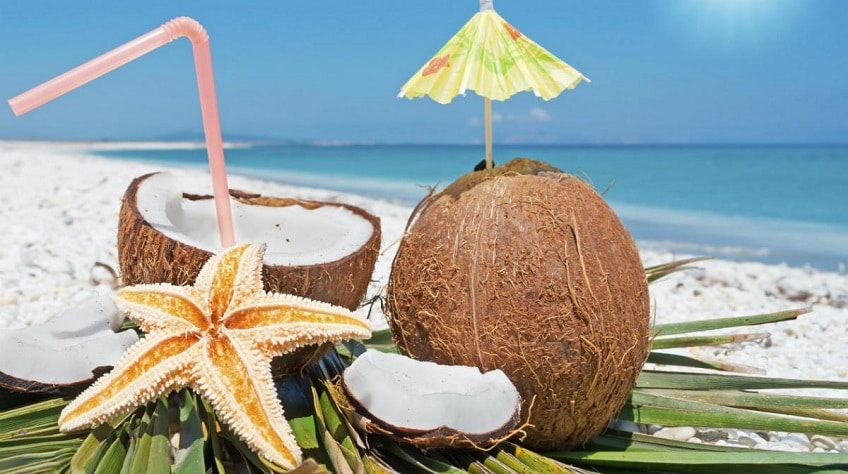
\includegraphics[width=0.5\textwidth]{imgs/coco_loco.jpg}
	\end{center}
\end{posterbox}

%====================================================================================%  
% left
\begin{posterbox}[name=assumption,column=0,row=1, below=intro]{Assumption}
	\textbf{Some mathematics stuff}
	\vspace{4cm}
	\begin{center}
		
\includegraphics[width=\textwidth]{imgs/coco_affe.jpg}
	\end{center}
	\vspace{5cm}
\end{posterbox}


%====================================================================================%  
% center
\begin{posterbox}[name=proof,column=1,row=1, below=intro]{Proof}
	\textbf{Something something in the month of May}
	\vspace{5cm}
\end{posterbox}

\begin{posterbox}[name=imgs,column=1,row=1, below=proof, bottomaligned=assumption]{Nice pictures}
	\textbf{This box is bottom aligned with "assumptions"}
\end{posterbox}

%====================================================================================%  
% right
\begin{posterbox}[name=alc,column=2,row=1, below=intro]{I don't know}
	\textbf{Schorle?}
	\begin{itemize}
		\item Warum gibts nur schöne Bilder mit rosé Schorle?
	\end{itemize}
	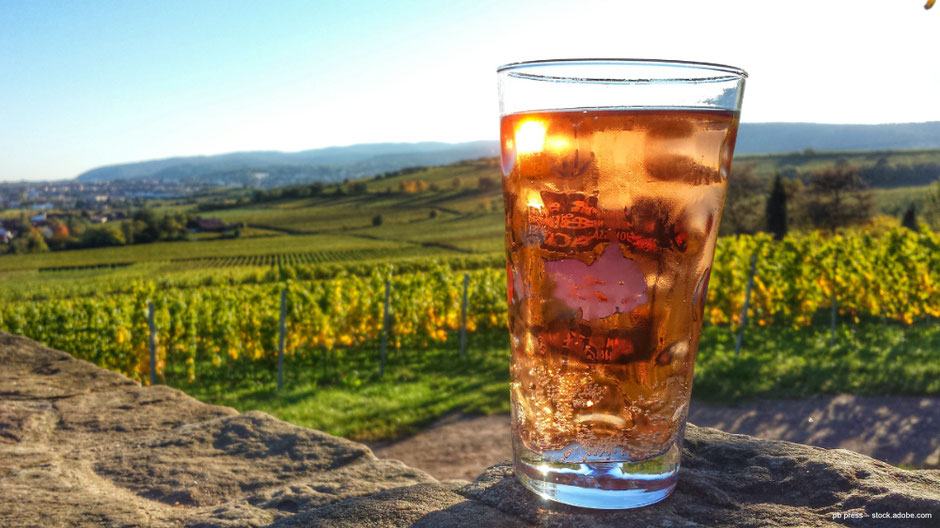
\includegraphics[width=\textwidth]{imgs/schorle.jpg}
	\vspace{3cm}
\end{posterbox}

\begin{posterbox}[name=rating ,column=2,row=1, below=alc, bottomaligned=assumption]{Rating}
	\begin{center}
		
\includegraphics[width=0.5\textwidth]{imgs/10_10.jpeg}
	\end{center}
\end{posterbox}


\end{poster}
\end{document}
